% vim: set tw=80 aw sw=2 sts=2 noet:
\documentclass{beamer}

%\includeonlyframes{c} % speeding up compilation speed during debug

\usepackage[utf8x]{inputenc} % diacritice
\PrerenderUnicode{ĂăâÂîÎșȘțȚ}
\usepackage[romanian]{babel}
\usepackage{hyperref}        % \url{http://...} | \href{http://...}{Nume Link}

% Pentru a include cod decomentati urmatoarele 3 linii
%\usepackage{color}			 % highlight
%\usepackage{alltt}			 % highlight
%\usepackage{code/highlight}	 % highlight

\mode<presentation>
%\usetheme{UEA}
%\usepackage{imperial-beamer}
\usetheme{SCS}

% Pentru a afisa (cont.) la slide-uri prea lungi split-uite pe mai multe pag
\setbeamertemplate{frametitle continuation}[from second]
% Pentru a modifica modul de afisare al numerelor de slide
\setbeamertemplate{footline}[frame number]

\title[SCS2010]{Analiza practică a simulatoarelor}
\subtitle{SCS2010: 21-22 Mai 2010}
\institute[CS]{Prof. Dr. Ing. Nume Prenume}
\author[A]{George Milescu (\texttt{george.milescu@gmail.com}) \\ 
  Dumitru Cristian (\texttt{dumitru.cristian@no-mail.me})}

\begin{document}

{
  % Schimbam fundalul aici pentru a avea slide-ul cu logo-urile
  % Nu știu momentan cum se face asta în template.
  \usebackgroundtemplate{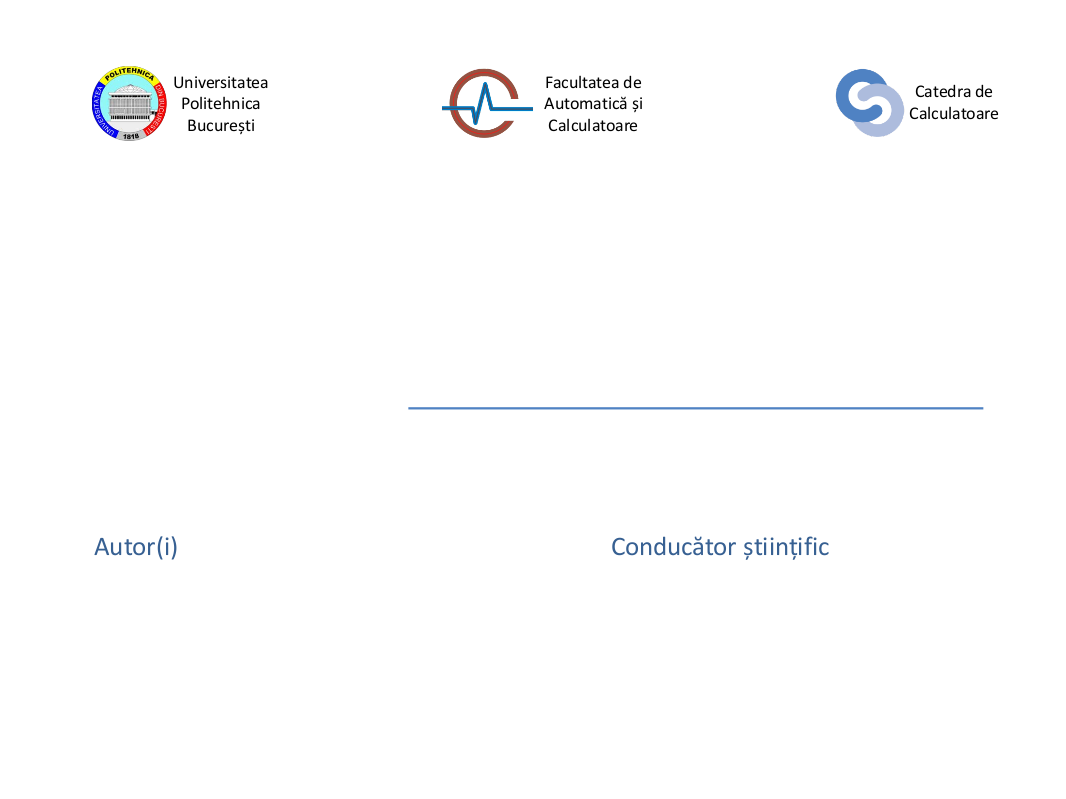
\includegraphics[width=\paperwidth]{title}}
  \frame{\titlepage}
}

\begin{frame}{Preambul}
  \begin{itemize}
    \item Introducere
    \item Primul capitol
    \item Al doilea capitol
    \item Al treilea capitol
    \item Concluzii
    \item Întrebări
  \end{itemize}
\end{frame}

\end{document}
